\documentclass[letterpaper,12pt]{article}
\usepackage[margin=1in,letterpaper]{geometry} % decreases margins
\usepackage{listings} % Listing for code block
\usepackage{amssymb}
\usepackage{amsmath}  % improve math presentation
\usepackage{graphicx} % Graphics library
\usepackage[spanish]{babel}
\usepackage[utf8]{inputenc}
\setlength\parskip{\baselineskip} % New line after each paragraph
\setlength\parindent{0pt} % Remove indent
    
\begin{document}
\lstset{language=Python}   

\title{Tarea 05}
\author{Martínez Flores Jorge Yael}
\date{\today}
\maketitle

\section{Algoritmos de aproximación}

La teoría de la NP-Completez nos ayuda a identificar problemas para los cuales
probablemente no existen algoritmos polinomiales que los resuelvan. Como no se
puede resolver en tiempo polinomial, necesitamos un algoritmo que se aproxime 
algoritmo menos a una solución optima, ahí es cuando entran los algoritmos 
de aproximación.

Un algoritmo de aproximación es un algoritmo usado para encontrar soluciones
aproximadas a los problemas de optimización. Un problema de optimización es un
problema que busca minimizar o maximizar el valor de una variable, es un 
problema que trata de calcular el valor máximo o mínimo de una función. A menudo
estan relacionados con los problemas $NP-hard$, como es casi imposible tener un
algoritmo eficiente en tiempo polinomial para resolver estos problemas, 
se intentan encontrar soluciones que no sean óptimas en tiempo polinomial.

Un algoritmo de aproximación puede ser determinista o no determinista. Si es 
no determinista y se ejecuta rápidamente, es común ejecutarlo varias veces para
poder elegir la mejor de las soluciones aproximadas. 

Los algoritmos de aproximación bien diseñados cuentan con un análisis formal que 
muestra que la diferencia entre su solución y la solución óptima es de un factor
constante, llamado Factor de aproximación. El factor de aproximación es menor 
que $1$ para maximización y mayor que $1$ para minimización. El valor extremo 
del factor sobre el conjunto de todos los ejemplares del problema es el índice 
de aproximación.

\section{Algoritmo de aproximación para Vertex Cover}

Sea una gráfica $G=(V,E)$ una gráfica, $C$ un conjunto, el siguiente es un algoritmo
de aproximación para la cubierta de vértices:
\begin{lstlisting}[escapeinside={(*}{*)}]

    def vertexCoverApproach(G):
        C = (*$\emptyset$*)
        E(*'*) = E
        while(E(*'*) != (*$\emptyset$*)):
            Sea (*$(u,v)$*) una arista arbitraria de G
            C = C (*$\cup \; (u,v)$*)
            Eliminar de E(*'*) cualquier arista que incida con (*u*) o (*v*)
        return C

\end{lstlisting}

Podemos ver que este algoritmo es polinomial ya que el ciclo \textit{while} toma
a lo más $n^2$ pasos al seleccionar arbitrariamente las aristas y eliminar las
aristas que tengan un extermo que incida en estos.

\subsection{Ejemplo del algoritmo de aproximación}

\begin{figure}[tph!]
    \centerline{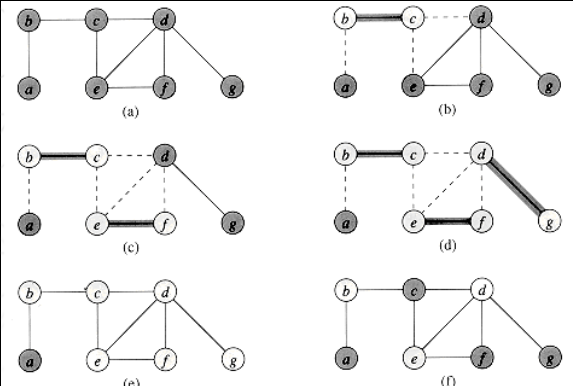
\includegraphics[totalheight=8cm]{img/vc.png}}
\end{figure}

\newpage

\textbf{Primera iteración}

\begin{figure}[tph!]
    \centerline{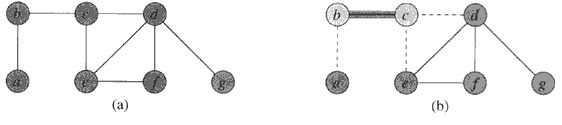
\includegraphics[totalheight=3cm]{img/vc1.jpg}}
\end{figure}

$C \neq \emptyset$

$E'= \{ (a,b), (b,c), (c,e), (c,d), (e,f), (e,d), (d,g) \}$

$E \neq \emptyset \Rightarrow$ Tomamos arbitrariamente la arista $(b,c)$

$C = C \cup \{b,c\}$ y se eliminan las aristas incidentes en $b$ y $c$ de $E'$

\textbf{Segunda iteración}

\begin{figure}[tph!]
    \centerline{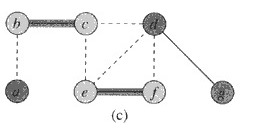
\includegraphics[totalheight=3cm]{img/vc2.jpg}}
\end{figure}

$E'= \{ (c,d), (e,f), (e,d), (d,g) \}$

$E \neq \emptyset \Rightarrow$ Tomamos arbitrariamente la arista $(e,f)$

$C = \{ b,c \} \cup \{ e,f \}$ y se eliminan las aristas incidentes en $e$ y 
$f$ de $E'$

\textbf{Tercera iteración}

\begin{figure}[tph!]
    \centerline{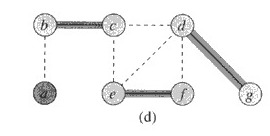
\includegraphics[totalheight=3cm]{img/vc3.jpg}}
\end{figure}

$E'= \{ (c,d), (d,g) \}$

$E \neq \emptyset \Rightarrow$ Tomamos arbitrariamente la arista $(d,g)$

$C = \{ b,c,d,f \} \cup \{ d,g \}$ y se eliminan las aristas incidentes en $d$ y 
$g$ de $E'$. Al final queda $E' = 0$

\textbf{Cuarta iteración}

\begin{figure}[tph!]
    \centerline{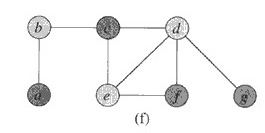
\includegraphics[totalheight=3cm]{img/vc4.jpg}}
\end{figure}


$E' = 0 \Rightarrow$ Regresa $C=\{ b,c,e,f,d,g \}$ 

\end{document}
    